\documentclass[xcolor=dvipsnames]{beamer}%[hyperref={pdfpagelabels=false}]{beamer}

\usepackage{polski}
\usepackage[utf8]{inputenc}
\usepackage{caption}

\usepackage{lmodern}
\usepackage{amsfonts}
\usepackage{hyperref}
\usepackage{amsmath}

%%%%%%%%%%%%%%%%Początek ustawień

\usepackage{beamerthemesplit}
\useoutertheme{infolines}
\useinnertheme{rounded}

%%%%%%%%%%%%%%%%%Koniec Ustawień

%%%%%%%%%%%%%%%%% SLAJD TYTUŁOWY

\title[Skrócony Wzór]{Presentation template}
\subtitle{Part II} 
\author[Skrócony Autor]{Łukasz Chojnacki}
\institute[WUST]{Chair of Cybernetics and Robotics \\ 
Faculty of Electronics \\ 
Wroclaw University of Science and Technology}
\date{\today}  %data

%%%%%%%%%%%%%%%%%



\begin{document}

\begin{frame}
\titlepage
\end{frame} 

\begin{frame}
\frametitle{Plan prezentacji}
\tableofcontents
\end{frame}

\section{Wstęp}
\subsection{Pierwszy merytoryczny slajd}
\begin{frame} %początek sladjdu
\frametitle{Nazwa Slajdu}
\framesubtitle{Podnazwa slajdu} %Opcjonalnie

\centering Zawartość tekstowa
		
\end{frame}%koniec slajdu

\subsection{Drugi merytoryczny slajd}
\begin{frame}
\frametitle{Pojawianie się puntków}
\framesubtitle{Bardzo efektowne}
	\begin{itemize}
		\item Pierwszy punkt
		\pause
		\item Drugi punkt
		\pause
		\item Trzeci punkt
	\end{itemize}
\end{frame}

\section{Koniec}
\subsection{Wstawianie Rysunku}
\begin{frame}
	\frametitle{Przepiękna i zjawiskowa}
	\centering \begin{figure}
   		       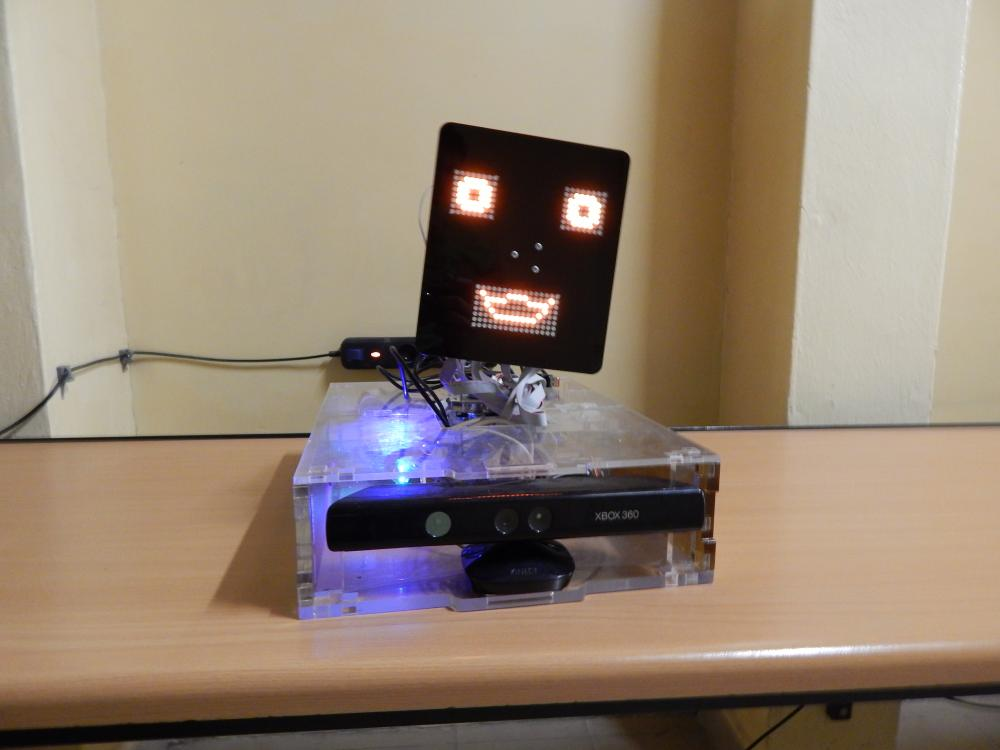
\includegraphics[height=5cm]{figure/balbina.jpg}
		       \caption{Balbina}
		       \end{figure}
\end{frame}

\subsection{Problemy}
\begin{frame}
\frametitle{Pomocy?}
	\begin{block}{Gdzie szukać porad}
	Pomocy szukajcie w internecie, to nie jest takie trudne : )
	\end{block}
\end{frame}
	
	

\end{document}